\section{Partial Differential Equations for the Solid Earth}
\subsection{Governing equations and boundary conditions}
Static deformation of the solid Earth over the time-scales of earthquake cycles is governed by the equilibrium equation and a constitutive relationship describing the material properties.  The standard assumption is that the Earth is linear elastic, defined on a sub-domain of $\mathbb{R}^3$.  While solutions to the 3D elasticity equations are the eventual target, 2D problems are considered in this work in order to sort out implementation details with reduced computational costs.  The 2D anti-plane shear problem \cite{antiplaneshear} is particularly ubiquitous in earthquake applications, where a vertical cross-section of a 3D problem (assuming invariance in one-direction) gives rise to an elliptic equation, where only one non-zero component of the displacement vector exists and depends on two spatial variables, namely,
\begin{equation}
    -\nabla \cdot \left({\mu} \nabla u\right) = f \quad \text{ for } (x, y) \in \Omega, 
    \label{eqn: 2D}
\end{equation}
where ${\mu}(x, y)$ is the spatially-varying shear modulus, $u$ is Earth's material displacement in the $z$-direction, and $f$ comprises body forces. In order to enable complex fault geometries and topography, we assume that $\Omega$ is a curved quadrilateral in $\mathbb{R}^2$, which enables extensions to arbitrary domains partitioned into computational blocks, \cite[e.g.][]{Kozdon2020HybridizedSF}. As \autoref{fig:trans}(a) illustrates, the boundary can be partitioned into four curves $\partial\Omega_i, \,\, i = 1, ..., 4$, where (for example), $\partial \Omega_3$ represents Earth's surface. The shear modulus $\mu(x, y)$ can vary in order to represent heterogeneities in the crust, for example, a sedimentary basin, which is known to trap waves, extend shaking, and increase earthquake magnitudes, \cite[e.g.][]{Boue2016}. 

In this work both Dirichlet and Neumann boundary conditions are considered for generality, as each appears in earthquake problems. For example Earth's free surface manifests as a Neumann condition and slow motion of tectonic plates is usually enforced via a Dirichlet condition \cite{Erickson2014}. As proof of concept, we consider boundary conditions
\begin{subequations}\label{eqn:2Dbc}
\begin{alignat}{3}
u &= g_{1},  &&\quad \partial\Omega_1,\\ 
u&= g_{2}, &&\quad \partial\Omega_2,\\ 
{\boldsymbol{n}} \cdot \mu\nabla u&=g_{3}, &&\quad \partial\Omega_3, \\
{\boldsymbol{n}} \cdot \mu\nabla u&=g_{4}, &&\quad \partial\Omega_4,
\end{alignat}
\end{subequations}
%
\noindent where vector $\boldsymbol{n}$ is the outward pointing normal to the domain boundary and $g_i, \,\, i = 1, ..., 4$ represent boundary data.  
\subsection{Coordinate Transformation}
In order to solve \autoref{eqn: 2D}-\autoref{eqn:2Dbc} with SBP-SAT methods, the domain $\Omega$ is transformed (via a conformal mapping) to the regular, square domain $(r, s) \in \bar\Omega = -1 \leq (r, s) \leq 1$, as in \autoref{fig:trans}(b). The transformed equations are given by
\begin{subequations}\label{eqn:2Dvar}
\begin{alignat}{3}
-\bar\nabla \cdot \left({\bf c} \bar\nabla u\right) &= Jf,  &&\quad{\text {for } (r, s) \in \bar\Omega}, \\ 
u &= g_{1},  &&\quad \text{face 1},\\ 
u&= g_{2}, &&\quad \text{face 2},\\ 
\hat{\boldsymbol{n}}^3 \cdot {\bf c}\bar\nabla u&=S^3_J g_{3}, &&\quad \text{face 3}, \\
\hat{\boldsymbol{n}}^4 \cdot {\bf c}\bar\nabla u&=S^4_J g_{4}, &&\quad \text{face 4},
\end{alignat}
\end{subequations}
where $\bar\nabla u = \left[\frac{\partial u}{\partial r}, \,  \frac{\partial u}{\partial s}\right]^T$, face $k$  for $k = 1, ... 4$ define the domain boundaries of $\bar{\Omega}$, given in \autoref{fig:trans}(b). $J >0 $ is the Jacobian and  $S^{k}_J$ is the surface Jacobian on face $k$.
Vector $\hat{\boldsymbol{n}}^k$ is the outward pointing normal to the face and $2 \times 2$ matrix ${\bf c}$ is symmetric positive definite (SPD) and encodes the variable material properties $\mu(x, y)$ and the coordinate transform, see \cite{Kozdon2020HybridizedSF, Erickson2022} for more details.

\begin{figure}
    \centering
     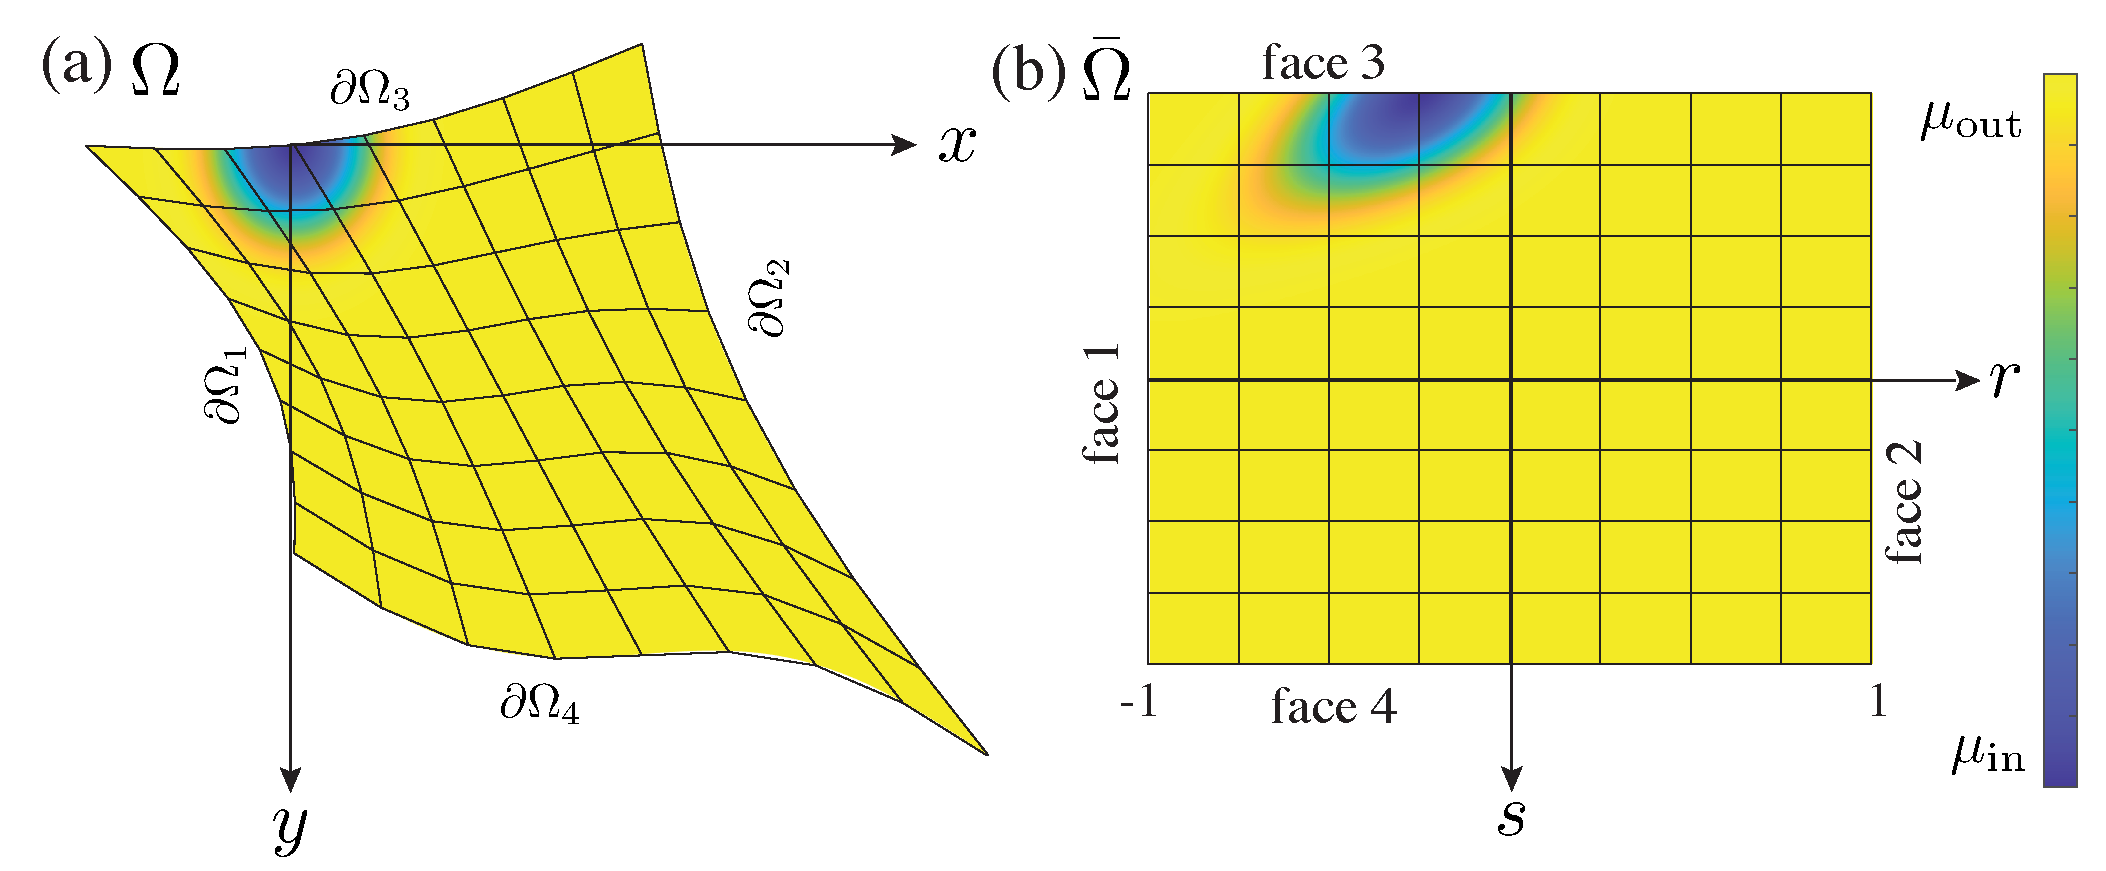
\includegraphics[width=\linewidth]{figures/grid_transformation.pdf}
    \caption{(a) Geometrically complex physical domain $\Omega$ with material stiffness that increases from $\mu_\text{in}$ within a shallow, ellipsoidal sedimentary basin, to stiffer host rock given by $\mu_\text{out}$.  (b) $\Omega$ is transformed to the regular, square domain $\bar{\Omega}$ via conformal mapping.} 
\end{figure}



\section{Problem Discretization}


\begin{figure}
    \centering
    %\includegraphics[width=\textwidth]{sparsity_patter_A.png}
     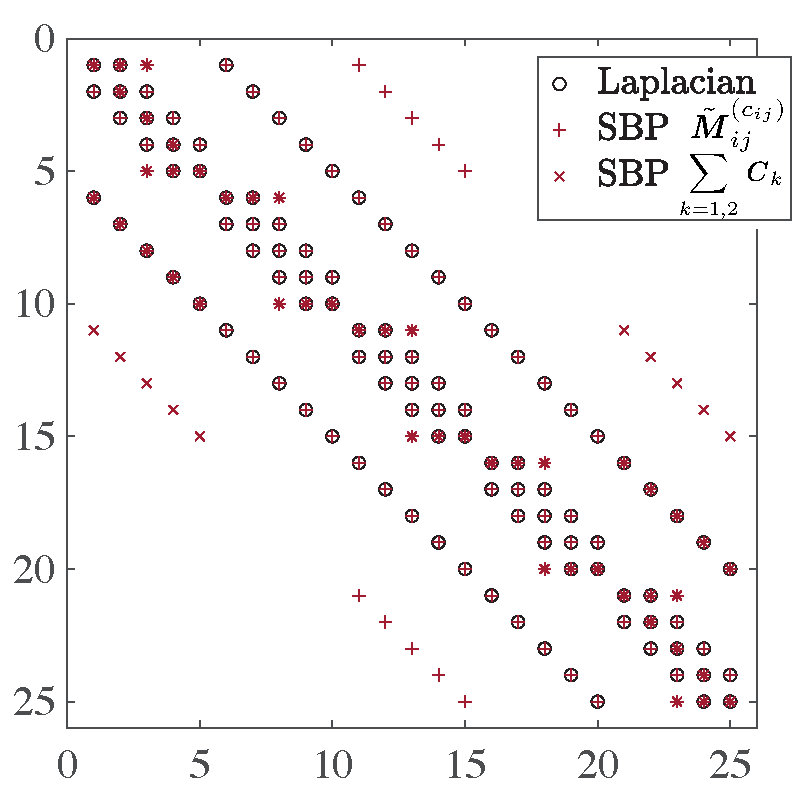
\includegraphics[width=\linewidth]{figures/iccs_spy_3.pdf}
    \caption{Sparsity pattern for matrix $\boldsymbol{A}$ with $N = 5$ grid points in each direction.  Traditional 5-point Laplacian stencil in black circles. Contributions to $\boldsymbol{A}$ are separated into contributions from the volume (red $+$) and from the boundary enforcement (red $\times$), so that contributions from both (red $\ast$) cancel any deviations from symmetry.} 
    \label{fig:sparsity_A}
\end{figure}

The SBP-SAT discretization to \autoref{eqn:2Dvar} is given by
\begin{equation}\label{eqn:2Ddiscrete}
    -\tilde{\boldsymbol{D}}_{ij}^{(c_{ij})}\boldsymbol{u} = \boldsymbol{Jf} + \sum_k \boldsymbol{p}_k
\end{equation}
where $\boldsymbol{p}_k$ are SAT vectors formed from the boundary condition on face $k$. To illustrate the structure of the SAT vectors, enforcing Dirichlet conditions on faces $k = 1, 2$ generates 

\begin{align}
\boldsymbol{p}_{k} &= \left(\boldsymbol{H} \otimes \boldsymbol{H}\right)^{-1}\left(\boldsymbol{G}_k^T  - \boldsymbol{L}_k^T \boldsymbol{H}_k {\boldsymbol \tau}_k   \right)\left(\boldsymbol{L}_k\boldsymbol{u} - \boldsymbol{g}_k\right), 
\end{align}


where matrix ${\bf G}_k = \hat{n}_i^k \boldsymbol{H}_k \boldsymbol{C}_{ij}^k \boldsymbol{B}_j^k$ computes the weighted derivative on face $k$. 
Matrix $\boldsymbol{\tau}_k$ = $\hat{n}^k_i \boldsymbol{C}^k_{ij}\hat{n}^k_j{\boldsymbol \Gamma}_k$, where ${\boldsymbol \Gamma}_k$ is the diagonal penalty matrix on face $k$ with sufficiently large components to ensure discrete stability, according to 

\begin{equation}
    {\boldsymbol \Gamma}_k \geq \frac{4}{h_\perp^k}{\bf I} + \frac{1}{h_\perp^k }{\bf P}_k,
\end{equation}

\noindent where 

\begin{equation}\label{eqn: minval}
{\bf P}_k = 
\begin{cases}
{\boldsymbol{C}}^{k}_{rr} ({\boldsymbol{C}}_{rr}^{k, min})^{-1}, \quad $k = 1, 2$,\\
{\boldsymbol{C}}^{k}_{ss} ({\boldsymbol{C}}_{ss}^{k, min})^{-1}, \quad $k = 3, 4$.
\end{cases}
\end{equation}
Here ${\boldsymbol{C}}^{k, min}$ is the minimum value of $c$ in the two points orthogonal to the boundary and $h_\perp^k$ is the grid spacing orthogonal to face $k$ \cite{Erickson2022}. 


Imposing Neumann conditions on faces $k = 3, 4$ corresponds to SAT vectors
\begin{align}
\boldsymbol{p}_{k} &= -\left(\boldsymbol{H} \otimes \boldsymbol{H}\right)^{-1}\boldsymbol{L}^T_k\left(\boldsymbol{G}_k \boldsymbol{u}  - \boldsymbol{H}_k \boldsymbol{S}_J^k \boldsymbol{g}_k\right).  
\end{align}



In order to render the linear system \autoref{eqn:2Ddiscrete} SPD, we multiply by $\left(\boldsymbol{H} \otimes \boldsymbol{H}\right)$ (the discrete equivalent of integrating over $\bar\Omega$ and discretizing the weak form). This process yields the final linear system 
\begin{equation}\label{eqn: final}
   \boldsymbol{A} \boldsymbol{u} = {\boldsymbol{b}} 
\end{equation} where
\begin{equation}\label{eqn:discrete}
\boldsymbol{A} = \tilde{\boldsymbol{M}}^{(c_{ij})}_{ij} + \sum_{k = 1, 2} \boldsymbol{C}_k,
\end{equation}
%

is SPD \cite{Erickson2022}, and matrices
\begin{equation}
    \boldsymbol{C}_k = -{\bf L}_k^T {\bf G}_k - {\bf G}_k^T {\bf L}_k + {\bf L}_k^T \boldsymbol{H}_k \boldsymbol{\tau}_k {\bf L}_k.
\end{equation}

Right-hand side vector $\boldsymbol{b}$ is given by
\begin{equation}
   {\boldsymbol{b}} = \left(\boldsymbol{H} \otimes \boldsymbol{H} \right)\left[\boldsymbol{J}\boldsymbol{f} + \sum_k \boldsymbol{K}_k \boldsymbol{g}_{k}\right]
\end{equation}
which encodes the source term and boundary data.  Here matrices $\boldsymbol{K}$ depend on boundary conditions; for those given in \autoref{eqn:2Dvar} they are
\begin{align}
    \boldsymbol{K}_1 &= \boldsymbol{L}_1^T  \boldsymbol{H}_1  {\boldsymbol\tau}_1 - \boldsymbol{G}_1^T \\
 \boldsymbol{K}_2 &= \boldsymbol{L}_2^T  \boldsymbol{H}_2  {\boldsymbol\tau}_2 - \boldsymbol{G}_2^T \\
  \boldsymbol{K}_3 &= \boldsymbol{L}_3^T \boldsymbol{H}_3\\
    \boldsymbol{K}_4 &= \boldsymbol{L}_4^T \boldsymbol{H}_4.
\end{align}
 Note that $\boldsymbol{A}$ includes contributions from both volume operators ($\tilde{\boldsymbol{M}}^{c_{ij}}_{ij}$) and from the SAT enforcement of boundary terms ($\boldsymbol{C}_k$), and differs from the traditional discrete Laplacian near all domain boundaries; see \autoref{fig:sparsity_A}. At Dirichlet boundaries (faces 1 and 2), $\boldsymbol{C}_k$ modifies the layer of three points normal to the face (i.e. the SAT imposition penalizes all points used in the computation of the derivative normal to the face).